% ===========================================================================
% ACT II -- Related Work and Positioning  (Ch. 2)   Slides 9-15
% Budget: 4 minutes. Chapter 2 is 42 KB of text; almost none of it belongs on
% screen. Resist surveying -- every slide here earns its place by narrowing.
% ===========================================================================

\actdivider{2}{Related Work}

% --- 9. The map ----------------------------------------------------------
\begin{frame}{Four Literatures, One Gap}
  \vspace{0.3em}
  \centering
  \scalebox{0.92}{%
    \only<1>{\litMap{0}}%
    \only<2>{\litMap{1}}%
  }

  \vspace{0.9em}
  \only<2>{%
    \begin{minipage}{0.88\textwidth}\small
      Each area solves part of the problem. None provides a model that is fast,
      built on the physics, \emph{and} usable for control on a train it was not
      trained on.
    \end{minipage}}
\end{frame}

% --- 10. Classical LTD ---------------------------------------------------
\begin{frame}{Classical Longitudinal Train Dynamics Simulation}
  \vspace{0.2em}
  \begin{columns}[T,onlytextwidth]
    \begin{column}{0.52\textwidth}
      {\footnotesize
      \begin{tabular}{@{}L{1.9cm}L{3.3cm}@{}}
        \toprule
        \textbf{Tool} & \textbf{Availability} \\
        \midrule
        TrainDy   & Consortium \\
        TOES      & Commercial (AAR) \\
        TEDS      & Publicly documented \\
        UM Train  & Commercial \\
        TDEAS     & Research / institutional \\
        CRE-LTS   & Research / in-house \\
        \bottomrule
      \end{tabular}}

      \vspace{0.7em}
      \srcline{Representative LTD tools; see Ch.~2 for full scope and origin.}
    \end{column}
    \begin{column}{0.44\textwidth}
      \begin{itemize}\setlength\itemsep{0.55em}
        \item Fidelity ranges from a single point mass to full constrained
              multibody dynamics.
        \item Most tools were developed as \textbf{in-house software}, with
              little published detail on numerical methods or assumptions
              {\scriptsize (Spiryagin et al., 2017)}.
        \item Computing coupler forces takes about \alert{65\% of solver
              run time} {\scriptsize (Wu \& Cole, 2015)}. The slack is the most
              expensive part to compute.
      \end{itemize}
    \end{column}
  \end{columns}
\end{frame}

% --- 11. Data-driven and hybrid in rail ----------------------------------
\begin{frame}{Data-Driven and Hybrid Modeling in Rail}
  \vspace{0.4em}
  \centering
  {\footnotesize
  \begin{tabular}{@{}L{3.6cm}L{3.7cm}L{4.9cm}@{}}
    \toprule
    \textbf{Approach} & \textbf{What It Predicts} & \textbf{What It Is Fixed To} \\
    \midrule
    Surrogate elements inside MBD {\scriptsize (Nie et al., 2018)}
      & Component response
      & One mechanical element, one model \\[0.3em]
    RNN surrogate as an FMU {\scriptsize (Zhou et al., 2023)}
      & Nominal simulator output
      & One track segment \\[0.3em]
    CNN + attention force estimation {\scriptsize (Zhang et al., 2024)}
      & Coupler force history
      & \alert{One coupler, one consist} \\[0.3em]
    In-trainNet {\scriptsize (2025)}
      & Forces at several couplers
      & Still needs per-configuration adaptation data \\[0.3em]
    Rescheduling surrogates {\scriptsize (Liu et al., 2024)}
      & Schedule quality
      & One operational context \\
    \bottomrule
  \end{tabular}}

  \vspace{1.0em}
  \begin{minipage}{0.92\textwidth}\small
    The third column is the key point. Each of these models is fast, but each is
    \textbf{tied to one specific} consist, coupler position or track section, and
    must be retrained when that changes.
  \end{minipage}
\end{frame}

% --- 12. Sequence models and neural operators ----------------------------
\begin{frame}{Sequence Models and Neural Operators}
  \vspace{0.3em}
  \begin{columns}[T,onlytextwidth]
    \begin{column}{0.47\textwidth}
      {\small\textbf{Long-Horizon Forecasting}}
      \begin{itemize}\setlength\itemsep{0.35em}
        \item[] {\footnotesize Informer, Autoformer, Temporal Fusion Transformer:
              attention models that handle long time series and combine fixed
              and time-varying inputs.}
      \end{itemize}
      \vspace{0.6em}
      {\small\textbf{Operator Learning}}
      \begin{itemize}\setlength\itemsep{0.35em}
        \item[] {\footnotesize FNO learns the solution of a differential
              equation in a form that works at any grid resolution. PINO adds a
              penalty when predictions violate the governing equations.}
      \end{itemize}
    \end{column}
    \begin{column}{0.49\textwidth}
      \begin{beamercolorbox}[wd=\linewidth,sep=6pt]{block body}
        {\footnotesize Why these models are a natural first choice, and why
         their structure does not fit this problem.}
      \end{beamercolorbox}
      \vspace{0.5em}
      \begin{itemize}\setlength\itemsep{0.5em}
        \item A transformer takes a \textbf{fixed-length input}: an 11-car and a
              150-car train must both be padded to the same length.
        \item \alert{The goal is a model that works for any train length.} A
              fixed input length works against that goal.
        \item PINO uses physics only as a \emph{training penalty}. In this work
              the physics is \emph{built into the model's calculation}.
      \end{itemize}
    \end{column}
  \end{columns}
\end{frame}

% --- 13. Graph networks for physical systems -----------------------------
\begin{frame}{Graph Networks for Physical Systems}
  \vspace{0.2em}
  \centering
  \scalebox{0.82}{%
    \only<1>{\mpStep{1}}%
    \only<2>{\mpStep{2}}%
    \only<3>{\mpStep{3}}%
  }

  \vspace{0.9em}
  \begin{minipage}{0.90\textwidth}\small\centering
    \only<1>{This model comes from work on message passing for particle and mesh
      simulations: Interaction Networks (Battaglia et al., 2016), Graph Network
      Simulators (Sanchez-Gonzalez et al., 2020), and MeshGraphNets
      (Pfaff et al., 2021).}
    \only<2>{Each edge (coupler) is updated from the two vehicles it connects.
      This mirrors the coupler force law $F_i = \phi_i(\delta_i, \dot\delta_i)$.}
    \only<3>{Each node (vehicle) is then updated from the edges attached to it.
      This mirrors the force balance
      $m_i \dot v_i = F_{\mathrm{ext},i} + F_{i-1} - F_i$.
      \textbf{The number of model parameters does not depend on $N$.}}
  \end{minipage}
\end{frame}

% --- 14. Probabilistic forecasting and calibration -----------------------
\begin{frame}{Probabilistic Forecasting and Its Reduced Role}
  \vspace{0.2em}
  \begin{columns}[T,onlytextwidth]
    \begin{column}{0.46\textwidth}
      \centering
      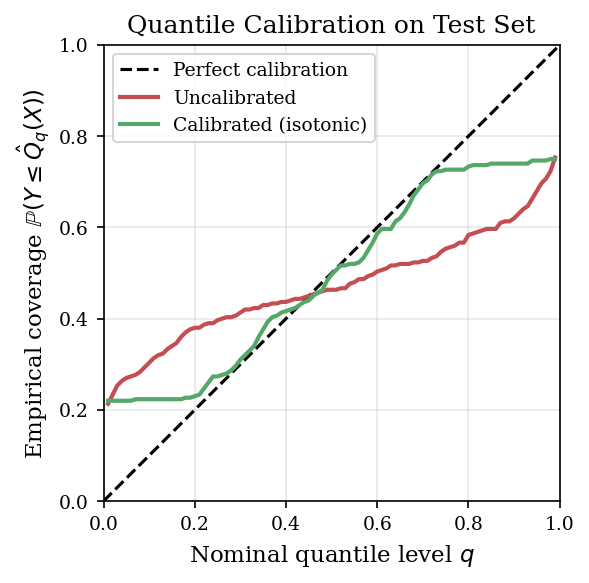
\includegraphics[width=\linewidth]{../figures/quantile_calibration.png}

      \vspace{0.3em}
      \srcline{The diagonal is perfect calibration.}
    \end{column}
    \begin{column}{0.50\textwidth}
      \begin{itemize}\setlength\itemsep{0.55em}
        \item The original plan was to predict probability distributions:
              quantiles and the chance of exceeding a limit.
        \item Calibration (honest probabilities) trades against
              \textbf{sharpness} (narrow ranges). Deep models are often
              overconfident on unfamiliar data.
        \item \alert{This thesis narrows that scope.} Uncertainty is used only as
              a \textbf{safety margin} the controller must respect.
      \end{itemize}
    \end{column}
  \end{columns}
\end{frame}

% --- 15. The gap ---------------------------------------------------------
\begin{frame}{The Gap, in One Table}
  \vspace{0.5em}
  \centering
  {\small
  \begin{tabular}{@{}p{5.4cm}ccc@{}}
    \toprule
    \textbf{Approach} & \textbf{Train-} & \textbf{Physics-} & \textbf{Differentiable} \\
                      & \textbf{Agnostic} & \textbf{Anchored} & \textbf{for Control} \\
    \midrule
    Classical LTD simulators
      & \yes & \yes & \no \\
    In-train force estimators
      & \no  & \no  & \yes \\
    Surrogate replacement inside MBD
      & \no  & \partly & \no \\
    Sequence and operator surrogates
      & \no  & \partly & \yes \\
    \midrule
    \textbf{This work}
      & \yes & \yes & \yes \\
    \bottomrule
  \end{tabular}}

  \vspace{1.2em}
  \begin{minipage}{0.90\textwidth}\small
    No existing rail surrogate is train-agnostic, built on the physics, and
    differentiable for control at the same time.
    \alert{Each existing approach meets at most two of the three.}
  \end{minipage}
\end{frame}
